\section{main.c File Reference}
\label{main_8c}\index{main.c@{main.c}}
{\tt \#include $<$stdio.h$>$}\par
{\tt \#include $<$stdlib.h$>$}\par
{\tt \#include $<$avr/io.h$>$}\par
{\tt \#include $<$avr/interrupt.h$>$}\par
{\tt \#include $<$avr/pgmspace.h$>$}\par
{\tt \#include \char`\"{}main.h\char`\"{}}\par
{\tt \#include \char`\"{}gpio.h\char`\"{}}\par
{\tt \#include \char`\"{}helpers.h\char`\"{}}\par
{\tt \#include \char`\"{}uart.h\char`\"{}}\par
{\tt \#include \char`\"{}leds.h\char`\"{}}\par
{\tt \#include \char`\"{}motor\_\-pwm.h\char`\"{}}\par
{\tt \#include \char`\"{}adc.h\char`\"{}}\par
{\tt \#include \char`\"{}gyro\_\-spi.h\char`\"{}}\par
{\tt \#include \char`\"{}accel\_\-capture.h\char`\"{}}\par
{\tt \#include \char`\"{}globals.h\char`\"{}}\par
{\tt \#include \char`\"{}monitor.h\char`\"{}}\par
{\tt \#include \char`\"{}irled\_\-pwm.h\char`\"{}}\par
{\tt \#include \char`\"{}stabilizer.h\char`\"{}}\par
{\tt \#include \char`\"{}transceiver\_\-mac.h\char`\"{}}\par


Include dependency graph for main.c:\begin{figure}[H]
\begin{center}
\leavevmode
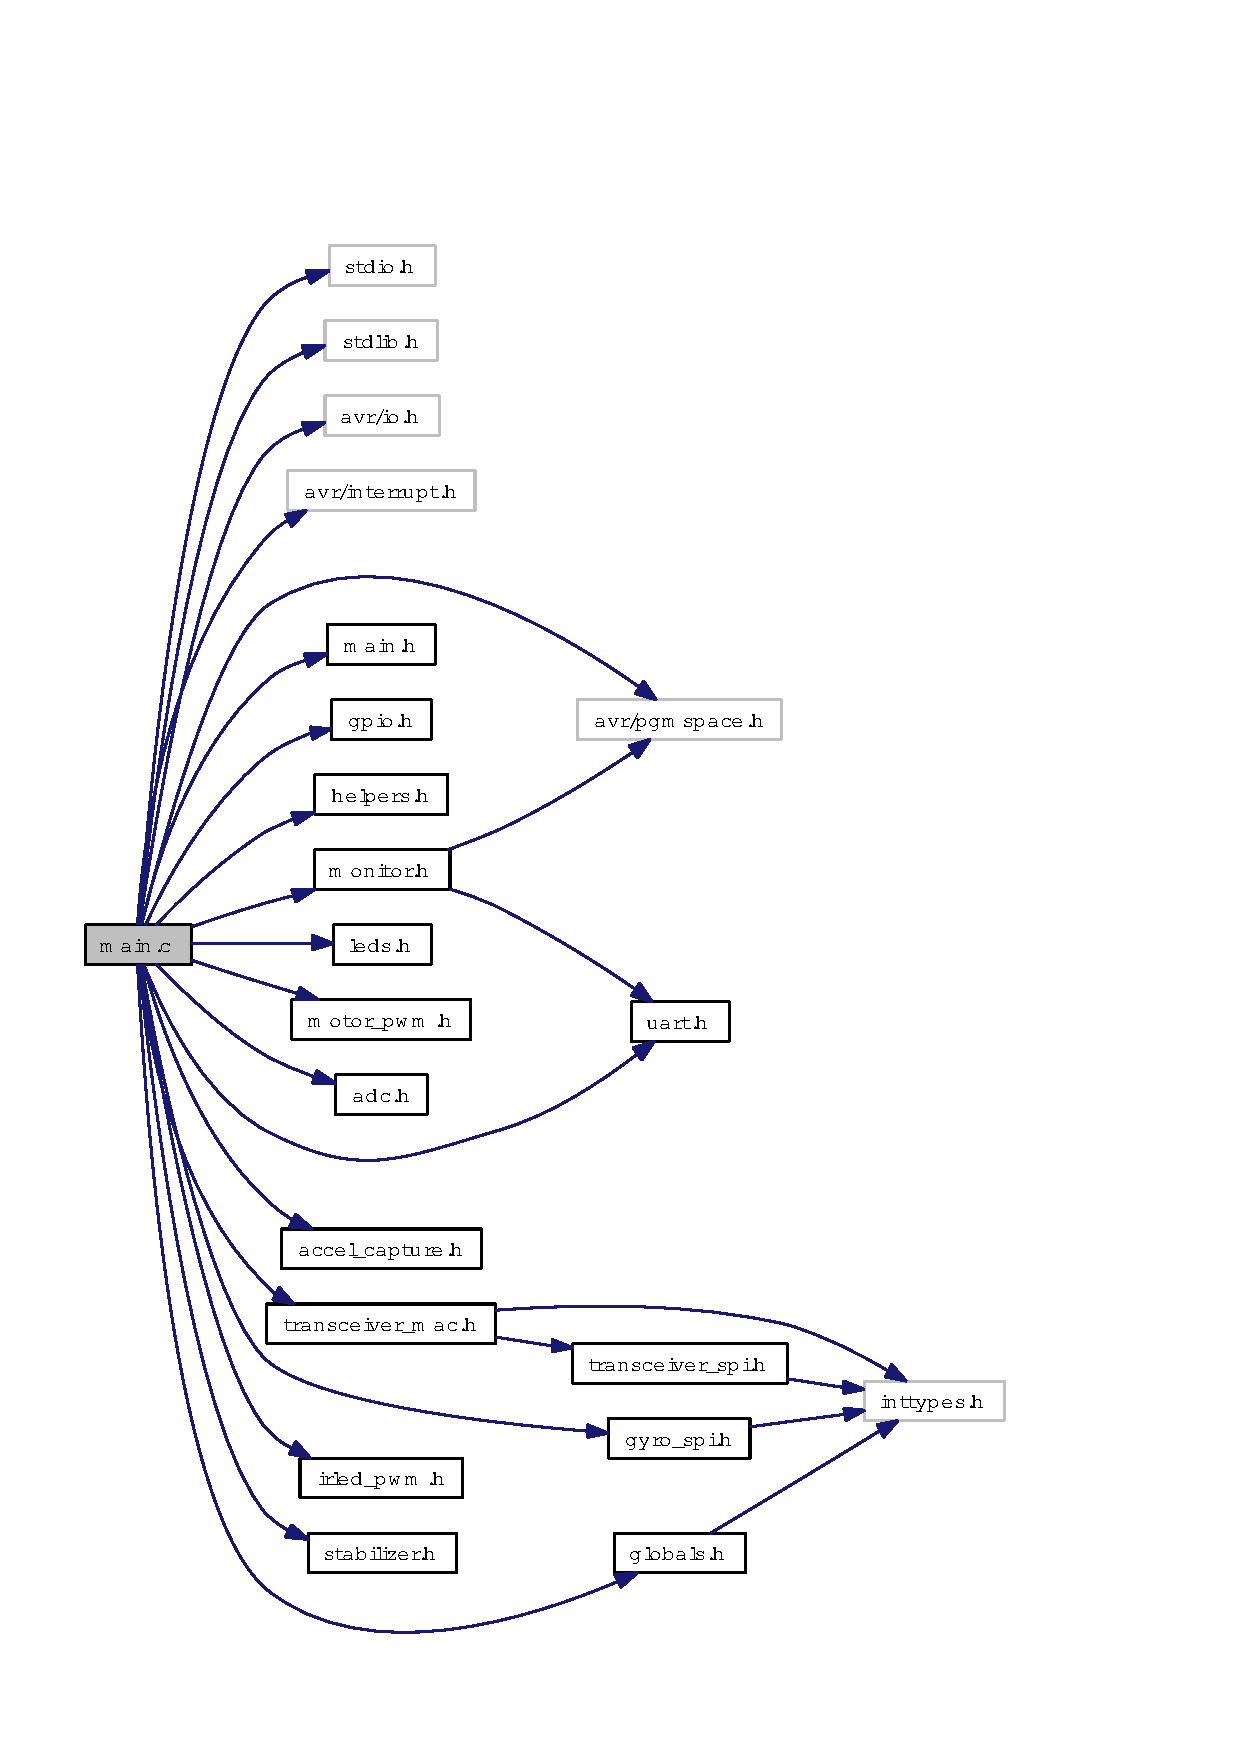
\includegraphics[width=243pt]{main_8c__incl}
\end{center}
\end{figure}
\subsection*{Functions}
\begin{CompactItemize}
\item 
void {\bf print\_\-status} ()
\item 
int {\bf main} (void)
\end{CompactItemize}
\subsection*{Variables}
\begin{CompactItemize}
\item 
const unsigned char {\bf random\_\-array} [1024]
\end{CompactItemize}


\subsection{Function Documentation}
\index{main.c@{main.c}!main@{main}}
\index{main@{main}!main.c@{main.c}}
\subsubsection{\setlength{\rightskip}{0pt plus 5cm}int main (void)}\label{main_8c_840291bc02cba5474a4cb46a9b9566fe}




Definition at line 163 of file main.c.

References disable\_\-motor1(), disable\_\-motor2(), init\_\-accel\_\-capture(), init\_\-adc(), init\_\-irled\_\-pwm(), init\_\-motor\_\-pwm(), init\_\-port\_\-directions(), init\_\-port\_\-values(), init\_\-uart(), MC13192\_\-init(), print\_\-status(), set\_\-led(), set\_\-motor1(), set\_\-motor2(), set\_\-motor\_\-pwm\_\-freq(), and uart\_\-puts\_\-P.

Here is the call graph for this function:\begin{figure}[H]
\begin{center}
\leavevmode
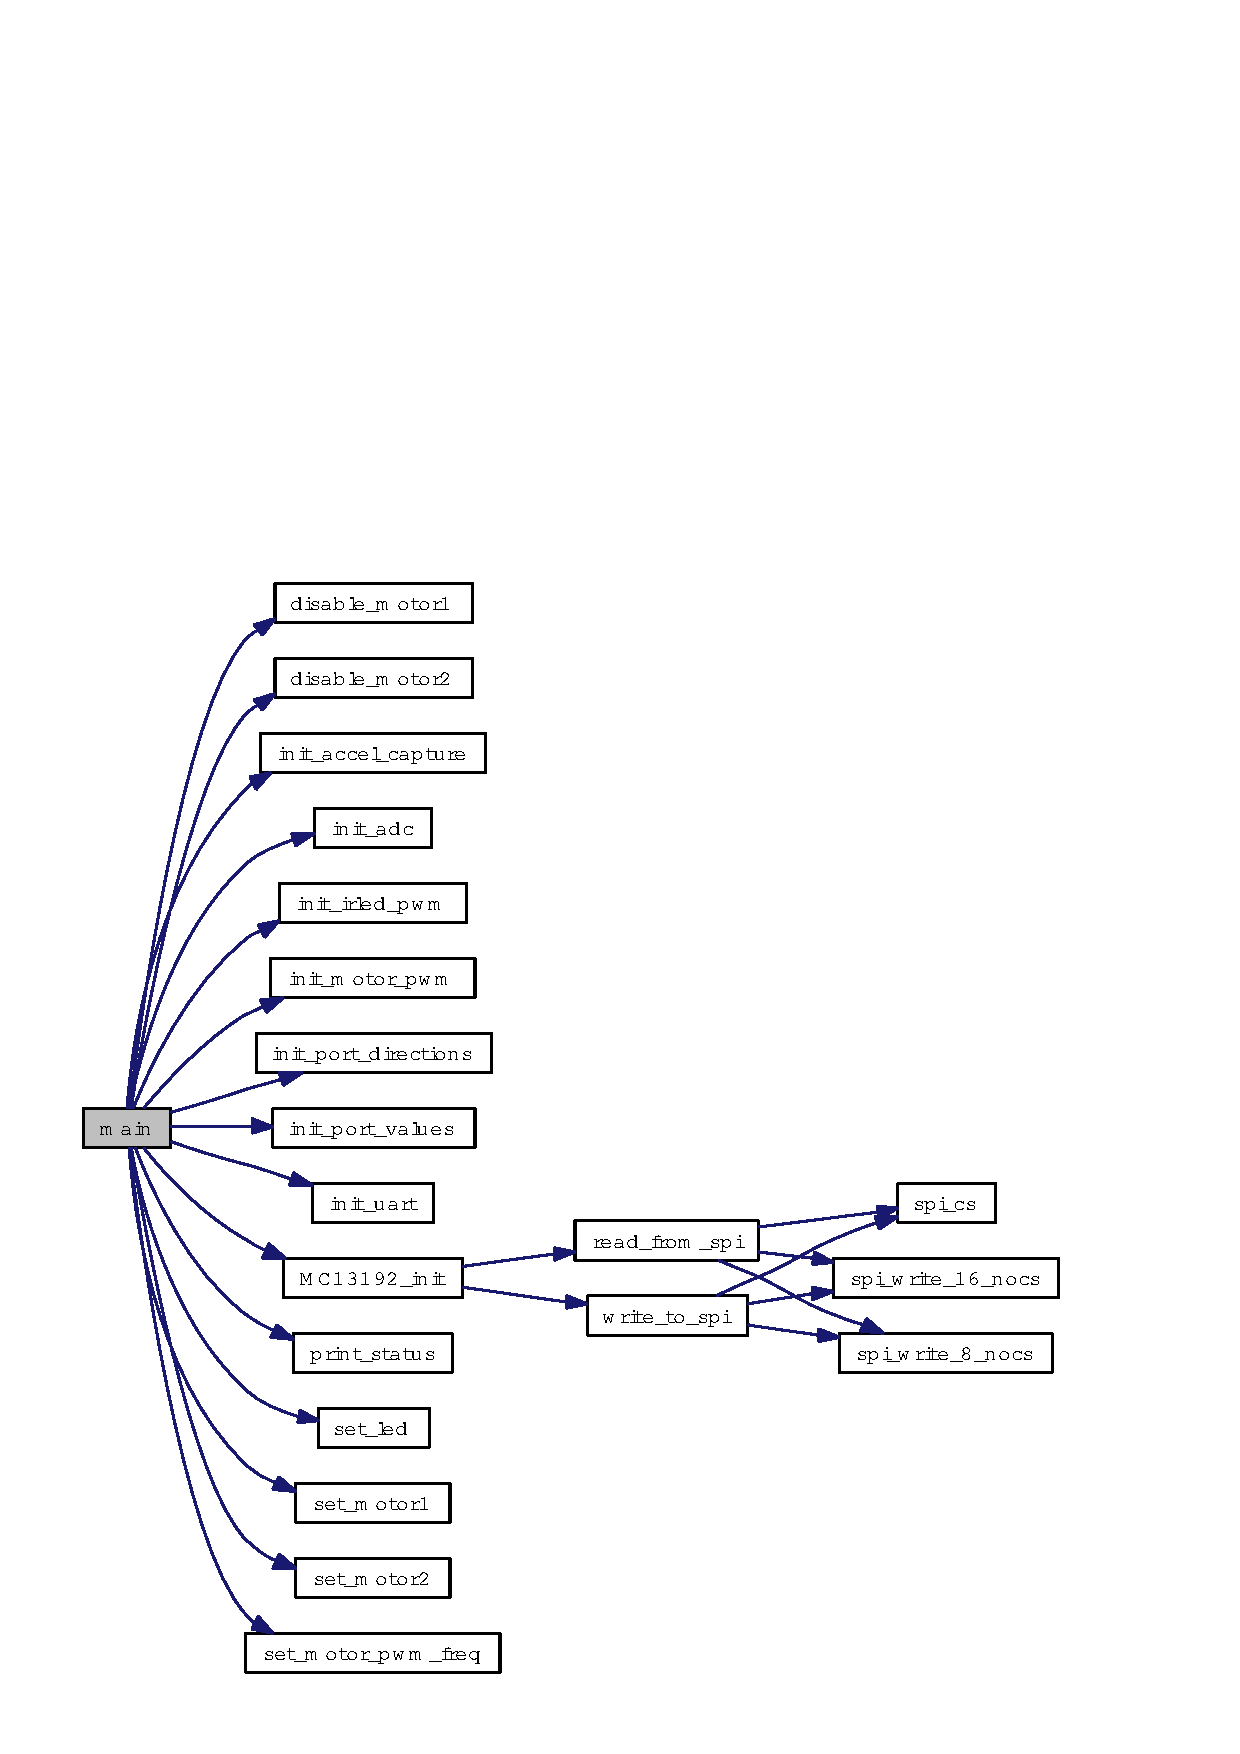
\includegraphics[width=256pt]{main_8c_840291bc02cba5474a4cb46a9b9566fe_cgraph}
\end{center}
\end{figure}
\index{main.c@{main.c}!print_status@{print\_\-status}}
\index{print_status@{print\_\-status}!main.c@{main.c}}
\subsubsection{\setlength{\rightskip}{0pt plus 5cm}void print\_\-status ()}\label{main_8c_8008fbbb8f369eeb0f452863fe664355}




Definition at line 156 of file main.c.

References uart1\_\-puts\_\-P, and uart\_\-puts\_\-P.

Referenced by main().

\subsection{Variable Documentation}
\index{main.c@{main.c}!random_array@{random\_\-array}}
\index{random_array@{random\_\-array}!main.c@{main.c}}
\subsubsection{\setlength{\rightskip}{0pt plus 5cm}const unsigned char {\bf random\_\-array}[1024]}\label{main_8c_3d904f51c6332f2482f0383ac9c918e6}




Definition at line 100 of file main.c.